\documentclass{../lib/llncs}
% Grundgröße 12pt, zweiseitig
% Standardpakete
% richtiges encoding fuer verschiedene compiler
\usepackage{iftex}
\ifPDFTeX
   \usepackage[utf8]{inputenc}
   \usepackage[T1]{fontenc}
   \usepackage{lmodern}
\else
   \ifXeTeX
     \usepackage{fontspec}
   \else
     \usepackage{luatextra}
   \fi
   \defaultfontfeatures{Ligatures=TeX}
\fi
% deutsche Silbentrennung
\usepackage[english]{babel}
\usepackage{amsmath}
\usepackage{cite}
\usepackage{float}
\usepackage{subfig}
\usepackage{changepage}
\usepackage{tabularx}

% Grafiken einbinden
\usepackage{graphicx}
\graphicspath{{../figures/}}

\usepackage{hyperref}
% tiefe des Inhaltsverzeichnisses
\setcounter{tocdepth}{2}

\usepackage{listings}
\usepackage{color}

\definecolor{dkgreen}{rgb}{0,0.6,0}
\definecolor{gray}{rgb}{0.5,0.5,0.5}
\definecolor{mauve}{rgb}{0.58,0,0.82}

\lstset{frame=tb,
  language=Python,
  aboveskip=3mm,
  belowskip=3mm,
  showstringspaces=false,
  columns=flexible,
  basicstyle={\small\ttfamily},
  numbers=none,
  numberstyle=\tiny\color{gray},
  keywordstyle=\color{blue},
  commentstyle=\color{dkgreen},
  stringstyle=\color{mauve},
  breaklines=true,
  breakatwhitespace=true,
  tabsize=3
}

\begin{document}

\title{Using deep reinforcment learning and self-play to master the game abalone}
\author{Ture Claußen, 1531067, \email{ture.claussen@stud.hs-hannover.de}}
\authorrunning{T. Claußen}
\institute{Hochschule Hannover Fakultät IV}

{\def\addcontentsline#1#2#3{}\maketitle} % Wird gebraucht, damit der Title nicht im Inhaltsverzeichnis steht

\begin{abstract}
  Perfect information games provide a great playing ground for the comparison of different algorithms, as they allow for direct comparison in a controlled environment. Whereas more classical approaches like minimax require human knowledge encoded in heuristics, modern approaches like (deep) reinforcement learning have excelled solely based on knowledge gained from self-play. To test how well this generalizes for other games, in the following, this is applied to the game abalone and compared with existing algorithms in a final tournament.
\end{abstract}


\section{Introduction}
Abalone is a fairly new game, that was devised in 1987 by Michel Lalet and Laurent Lévi. Nevertheless, with more than four million global sales it has established itself as a classic game \cite{noauthor_abalone_2020}. Abalone is a two-player game consisting of a hexagonal board with 61 fields and 14 marbles for black and white respectively. The abstract nature of the game requires the player to plan ahead and find the right strategy in the plethora of moves.

As it is a two-player perfect information game it can be solved, in theory, by backward induction. However, in search of the optimal move it is not possible to expand all of the possible paths the game could take, even for modern computers. Hence, more sophisticated approaches for navigating the search space are needed. This simple yet complex nature of this type of game make it very suitable for theoretic analysis. \cite[p. 1]{demichelis_simple_2004}

Ranging from game theory to artificial intelligence, games have sparked theoretical inquiry with many real world applications in economics, psychology, mathematics, neuroscience and many more. \cite[pp. 46]{russell_artificial_2021}
% 1)WHY
% 2)WHAT

\section{Background}
The comparison between a human's and a computer's proficiency in a game is particularly interesting as it allows for very tangible conclusions about the current state of affairs. IBM's "Deep Blue" (DB) win against Gary Kasparov \cite{higgins_brief_2017} in chess caused big public interest just as the win of "AlphaGo" (AG) against Lee Sedol \cite{deepmind_match_nodate} in the game Go. These two milestones also represent a shift in technology. Whereas Deep Blue relied on minimax, AlphaGo relied on a combination of multiple deep neural nets trained in self-play. \cite{silver_mastering_2017}

Building on this success DeepMind, the company behind AG, further improved the architecture. "AlphaGo Zero" and the generalization "AlphaZero" (AZ) learn \textit{tabula rasa}, without the help of human knowledge and surpassed the performance of AG significantly. Since then the architecture has been applied to Chess, Shogi and Atari games by removing the last piece of human knowledge in the system: The rules of the game. \cite{schrittwieser_mastering_2020}

There is a formidable body of work regarding classical game-playing agents and some based on learning algorithms. The most significant contributions are:

\begin{enumerate}
  \item "Algorithmic fun-abalone" (2002) Considers foundational heuristics for the game and analyzes minimax and its refinements in the form of (heuristic) alpha-beta pruning. Furthermore it sheds light on the performance differences between those. \cite{aichholzer_algorithmic_2002}
  \item "Abalearn: Efficient Self-Play Learning of the game Abalone" (2003) Utilizes TD-Learning to create a self-learning agent that is on par with intermediate players. \cite{campos_abalearn_2003}
  \item "A Simple Intelligent Agent for Playing Abalone Game: ABLA" (2004) Implementation of a game-playing agent with minimax, alpha-beta pruning and some custom heuristics. The evaluation of the performance is done by comparing the agent to existing software in the form of ABA-PRO and RandomSoft.\cite{ozcan_simple_2004}
  \item "Constructing an abalone game-playing agent" (2005) Provides a very thorough explanation and analysis of the game's fundamentals, such as the state space, rules and positions. In regards to the alpha-beta pruning it also explains strategies for ordering the nodes and performance concerns. \cite{lemmens_constructing_2005}
  \item "Implementing a computer player for abalone using alpha-beta and monte-carlo search" (2009) This master thesis is a very exhaustive analysis of the game, alpha-beta pruning and Monte Carlo tree search, conferring many of the previous results. \cite{chorus_implementing_2009}
\end{enumerate}

Considering the date of the publications interest into the game has cooled off. However there are some smaller student publications of the more recent years that apply Q-Learning and TD-Learning. \cite{mizrachi_introduction_2017} \cite{lee_abalone_2005}

\section{Aims and objectives}
The thesis has the objective to modify the architecture of AlphaZero (c.f. fig. \ref{alphazero_architecture} \& \ref{alphazero_architecture_details}) such that it can applied to the game of Abalone. As the computational resources are not as vast as those of Google, it has to be evaluated how the architecture works on smaller networks with less training duration.

In detail the steps to achieving that objective are to:

\begin{itemize}
  \item adapt the architecture of AlphaZero and to implement it,
  \item implement a self-training pipeline,
  \item answer the question: \textit{How well does the architecture of AlphaZero generalize?}
\end{itemize}

\section{Methodology}
A key element for the success of AlphaZero might advancement in computational resources, wherefore this project requires sufficiently powerful hardware to adequately replicate the conditions. For smaller scale testing in the initial phase there is the possibility to use a personal workstation with a GTX 1660S and 6 core processor. Moreover, the Hochschule Hannover might be able to provide a more powerful workstation. For the larger scale and final experiments an application for the usage of Google's TPU Research Cloud has been successfully granted. It allows for the usage of "up to 5 on-demand Cloud TPU v3 devices, 5 on-demand Cloud TPU v2 devices, and 100 preemptible Cloud TPU v2 devices for free for 30 days" \cite{noauthor_tpu_nodate}. This can be combined with the free \$300 credit for new Google cloud accounts. \cite{noauthor_free_nodate}

To assess the performance of the trained algorithm (variants) it will be compared with other algorithms in a tournament. All of the algorithms devised in related papers are not freely accessible wherefore access has been requested via email. As baseline there are the implementations created in a previous project \cite{noauthor_ture_nodate} which would need further improvement to be more competitive. Namely that would be a parallelization of the Minimax algorithm by switching to principal variation splitting or an alternative that preserves pruning. \cite{gao_multithreaded_nodate}

\section{Timeline}
\begin{table}
  \begin{center}
    \begin{tabularx}{\textwidth}{ | X | X | }
      \hline
      Week    & Item                                                                                                 \\
      \hline
      [-2, 1) & Foundational courses on usage of tensorflow and notation in RL                                       \\
      \hline
      [1, 2]  & Reading and gathering of related material                                                            \\
      \hline
      [3 - 4] & Planning of software, including research on more suitable game engine                                \\
      \hline
      [5]     & Implementation of first design and small tests                                                       \\
      \hline
      [6]     & Iteration over first design and preparation for distribution of training across multiple TPUs  tests \\
      \hline
      [7]     & Preparation of final experiment   tests                                                              \\
      \hline
      [8 - 9] & Training of large model and tournament   tests                                                       \\
      \hline
      [10-12] & Final writing, printing and submission                                                               \\
      \hline
    \end{tabularx}
  \end{center}
  \label{timetable}
\end{table}

\section{Preliminary table of contents}
\begin{enumerate}
  \item Introduction
\end{enumerate}

\newpage
\appendix

\section{AlphaZero architecture}

\begin{figure}[!h]
  \centering
  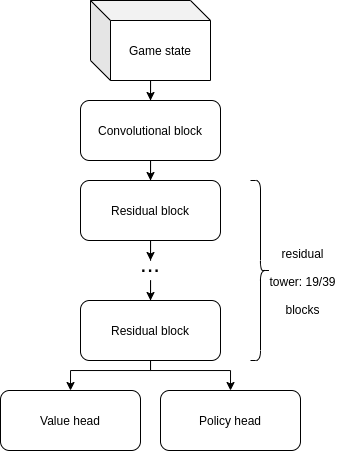
\includegraphics[height=8cm, keepaspectratio]{alphazero_architecture_network.png}
  \caption{The coarse architecture of AlphaZero \cite{silver_mastering_2017}}
  \label{alphazero_architecture}
\end{figure}

\begin{adjustwidth}{-5in}{-5in}% adjust the L and R margins by 1 inch
  \begin{figure}[!h]
    \centering
    \subfloat[Residual block]{
      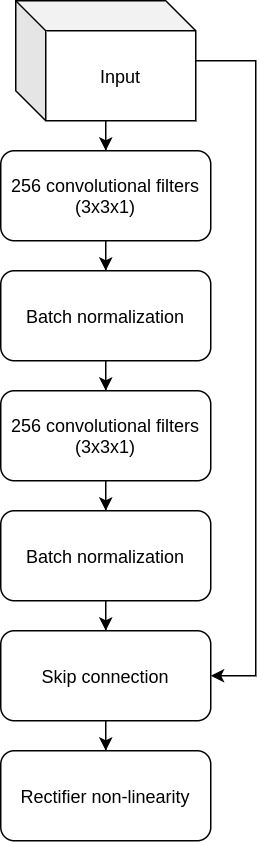
\includegraphics[width=3.9cm, keepaspectratio]{alphazero_architecture_residual_block.png}
    }
    \hfill
    \subfloat[Policy head]{
      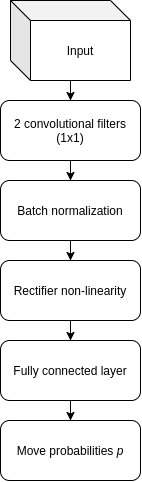
\includegraphics[width=3cm, keepaspectratio]{alphazero_architecture_policy_head.png}
    }
    \hfill
    \subfloat[Value head]{
      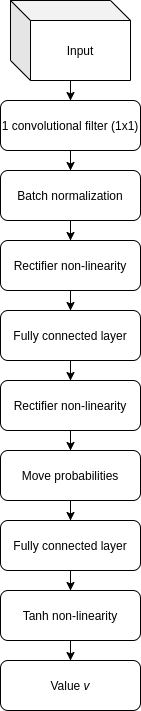
\includegraphics[width=3cm, keepaspectratio]{alphazero_architecture_value_head.png}
    }
    \caption{The different components of AlphaZero in detail \cite{silver_mastering_2017}}
    \label{alphazero_architecture_details}
  \end{figure}
\end{adjustwidth}
\newpage
% Literatur
\bibliographystyle{../lib/splncs04.bst}
\bibliography{../ref.bib}
\end{document}